\documentclass[11pt,dvipdfm]{article}

% Latex Packages
\usepackage{deauthor,times,graphicx}
\usepackage{multirow}
\usepackage{url}
\graphicspath{{aminedadoun/}}

\begin{document}

\title{Optimizing Email Marketing Campaigns in the Airline Industry \\ using Knowledge Graph Embeddings}

\author{
  Amine Dadoun\\
  EURECOM, Sophia Antipolis, France\\
  Amadeus SAS, Biot, France\\
  \texttt{amine.dadoun@eurecom.fr}
  \and
  Rapha{\"{e}}l Troncy\\
  EURECOM, Sophia Antipolis, France\\
  \texttt{raphael.troncy@eurecom.fr}
  \and
  Michael Defoin Platel\\
  Amadeus SAS, Biot, France\\
  \texttt{michael.defoinplatel@amadeus.com}
  \and
  Riccardo Petitti\\
  Amadeus SAS, Biot, France\\
  \texttt{riccardo.petitti@amadeus.com}
  \and
  Gerardo Ayala Solano\\
  Amadeus SAS, Biot, France\\
  \texttt{gerardo.ayalasolano@amadeus.com}
}

\maketitle

\begin{abstract}
The use of email marketing campaigns in e-commerce is an essential aspect for driving sales and establishing or maintaining good customer service. However, ensuring their success in the airline industry is challenging, and the risk is high that the marketing campaign content is not suited to the needs of specific travelers. The traveler may rapidly feel spammed and the offer content promoted via emails may even be no longer accessed. Consequently, the use of personalised recommender systems for email marketing campaigns becomes essential to build user loyalty and to increase offer conversion. Recently, the use of knowledge graphs has proven to be an effective way to recommend products. In this work, we propose an approach that leverages knowledge graph embeddings to better target the right audience in email marketing campaigns for airline products recommendation. We conduct extensive experiments to compare our approach with the currently in-production rule-based system used by airline marketers and a supervised machine learning model based on handcrafted features as another baseline. The results suggest that the use of knowledge graph embeddings is the most effective approach.
\end{abstract}


\section{Introduction}
\label{sec:introduction}
With the digital transformation of retail commerce from physical sale points to virtual stores, recommender systems have shown their value in easing the search and purchase decision process of customers who are facing an ever increasing amount of products~\cite{Dadoun21}. In order to embrace e-commerce techniques and boost their revenues, some airlines are using the so-called Amadeus Anytime Merchandizing (AAM) Notification System \footnote{\url{https://amadeus.com/en/portfolio/airlines/anytime-merchandising}} which is an IT solution that allows airline marketers to effectively define, deploy, monitor and adjust airline email marketing campaigns sent to the travelers in real-time. Customized notifications can be defined and sent to travelers, after booking a flight, to suggest them additional services to buy (e.g. extra baggage, specific meal, preferred seat) called ancillaries. The solution acts as a bridge between the travelers retailing touchpoints and the airline's service and delivery system. As shown on the left side of Figure~\ref{fig:TKE-approach}, when using this solution, the airline marketer can choose the appropriate time \textbf{when} to send the notification (e.g. 5 days before departure), \textbf{what} product to recommend (e.g. Leg Space Seat), \textbf{how} to send the offer (e.g. via an Email) and to \textbf{whom} this offer should be sent (matching targeting criteria).

Despite all the functionalities included in the AAM Notification System, it is difficult for an airline to find the optimal audience to target for a given offer. We conducted an analysis of historical sales triggered by some notification campaigns during the period 14 May 2019 - 17 Dec 2019 ran by one of our partner airlines and we observed a poor conversion of the notification offers (Section ~\ref{sec:campaign-analysis}). This is partly due to the challenging decision-making process that an airline marketer faces when it comes to deciding which values (belonging to broad ranges) are appropriate for the criteria to be used (e.g. sending time, flight itineraries, flight departure point, etc.). Targeting customers with unsolicited notifications can be counter-productive and lead to adversarial effects on customer loyalty if done incorrectly. It is therefore critical to identify the customers that we  expect to react positively to an advertised service in order to avoid spamming them with non-personalized emails. This problem can be seen as an inverse recommendation scenario, i.e. recommending a user to an item.

\begin{figure}[htbp]
  \centering
  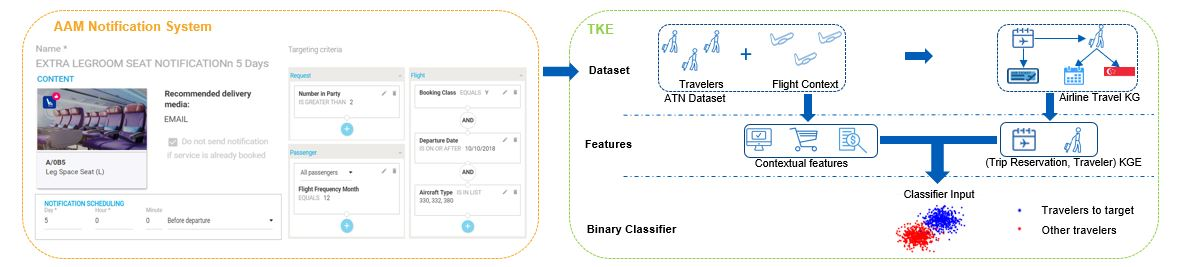
\includegraphics[width=\linewidth, height=4 cm]{figs/AAM_Notif_TKE-approach.PNG}
  \caption{On the left side: AAM Notification System. On the right side: Flowchart of our proposed TKE framework. Notification dataset used in this study is generated from the AAM Notification system. Contextual features include booking context (e.g. number of passengers, date of departure, etc.), notification information (e.g. media used to send the notification, time of notification, etc.).}
  \label{fig:TKE-approach}
\end{figure}

Inspired by recent works that have illustrated the effectiveness of using knowledge graph embeddings~\cite{Palumbo18, Sun18, Palumbo20} and gradient boosting algorithms~\cite{Pawel19, Schifferer20} for item recommendation, we propose the \textbf{T}ravel \textbf{K}nowledge Graph \textbf{E}mbeddings for email marketing campaigns (TKE) framework to better target the audience for a service the airline wishes to recommend through email marketing campaigns (Figure~\ref{fig:TKE-approach}). In this paper, we made the following contributions:
\begin{enumerate}
    \item We design and develop a Knowledge Graph using Semantic Web technologies to represent the travelers past trips as well as to semantically enrich airline products. 
    \item We learn vector representations of travel entities via knowledge graph embedding algorithms and we leverage gradient boosting algorithms to compute prediction scores to better target the audience in email marketing campaigns.
    \item We perform an empirical comparison of our approach with the current in-production rule-based system as well as with an hypothetical classical machine learning approach using handcrafted features on a real-world production dataset.
\end{enumerate}

The paper is organized as follows. Section~\ref{sec:related-work} provides a literature review of the related work. Section~\ref{sec:data-problem-formulation} introduces some preliminary concepts, the recommendation problem, the dataset and the knowledge graph used to conduct this work. In Section~\ref{sec:approach}, we describe both our TKE approach as well as a machine learning model using handcrafted features as another baseline. In Section~\ref{sec:experiments}, we present the experiments we carried out and we demonstrate the effectiveness of our approach. Finally, in Section~\ref{sec:conclusion}, we give some conclusions and we outline some future works.

\section{Related Work}
\label{sec:related-work}
This section provides a literature review of the research conducted on email marketing campaigns in the e-commerce and tourism domains. We also present state-of-the-art methods of knowledge graph embedding algorithms and the use of gradient boosting algorithms for recommender systems. 

\subsection{Email Marketing Campaigns}
\label{sec:sota-email-marketing}
Emails allow marketers to send messages to their customers at very low cost. They generally generate faster responses and create an opportunity for interactive communication with customers~\cite{Chittenden2003}. In~\cite{Sahni17}, the authors analyze 70 randomized field experiments and find that email promotions not only increase customers' average purchase spending during the promotion window but also carry over to the week after the promotion expires. In our study, we will focus on personalized email marketing campaigns. In~\cite{Abakouy17}, the authors performed an empirical comparison of supervised machine learning models based on decision tree and logistic regression algorithms in order to improve the open rate and conversion rate of email marketing campaigns. In~\cite{Deligiannis2020}, the authors propose to use transactional features and instant messaging metadata to train a boosting tree regression algorithm to timely anticipate the needs of consumers in order to increase their level of engagement as well as the rate at which they repurchase products.

In the tourism domain, even if widely used, limited research is conducted on email marketing campaigns. In~\cite{Tamho05}, the authors found that customers' favourite emails contain special offers, discounts and coupons as well as real-time communication tools. When customers perceived these emails as meeting their personal preferences, they developed a strong relationship with the sender. In~\cite{Yang19}, the authors demonstrated that the personalization, interactivity and price were important predictors of the possibility of revisiting the same accommodation. To the best of our knowledge, we are the first to propose a supervised machine learning approach to enable personalized email marketing in the airline travel industry.

\subsection{Knowledge Graph Embeddings}
\label{sec:sota-KGE}
A knowledge graph embedding (KG embedding) is a representation of a knowledge graph (KG) component into a continuous vector space. The objective of learning those embeddings is to ease the manipulation of graph components (entities, relations) for prediction tasks such as entity classification, link prediction or recommender systems.

In~\cite{Wang18}, the authors classified the learning algorithms into two main categories namely translational distance models and semantic matching models.

For the first category, TransE~\cite{bordes13} is often mentioned as the most used translational distance model. TransE represents both entities and relations vectors in the same space $R^{d}$. Given a fact (h, r, t), the relation is interpreted as a translation vector r so that the embedded entities h (head) and t (tail) can be connected by r with low error, i.e., $h+r \approx t$ when (h, r, t) holds. TransH~\cite{Wang14} introduces relation-specific hyperplanes, each relation r being represented on a hyperplane as $w_{r}$ its normal vector. TransR~\cite{Yankai15} follows the same idea as TransH, but instead of projecting the relations into a hyperplane, it proposes to create a specific space per relation.

In the second category, semantic matching models exploit similarity-based scoring functions. In~\cite{Maximilian11}, the authors associate each entity with a vector to capture its latent semantics. Each relation is represented as a matrix that models pairwise interactions between latent factors. The score of a fact (h, r, t) is defined by a bi-linear scoring function minimized through tensor factorization based on ALS optimization technique.

Palumbo et al.~\cite{Palumbo17} propose to use property-specific KG embeddings generated from node2vec algorithm~\cite{Aditya16} in order to compute relatedness scores between items and users. Similarly, we propose to use translational distance and semantic matching models to generate embeddings and to use them as latent features of a gradient boosting algorithm.

\subsection{Gradient Boosting Algorithms}
\label{sec:sota-gradient-boosting}
Gradient boosting is a machine learning technique for regression and classification problems, which produces a prediction model in the form of an ensemble of weaker prediction models. 

In~\cite{Pawel19}, the authors used multiple additive Regression Trees (Dart) which is an ensemble model that uses boosted regression trees and handles the overspecialization. Their approach for online accommodation recommendation ranked $1^{st}$ in the famous RecSys 2019 Challenge\footnote{\url{https://recsys.acm.org/recsys19/challenge/}}. In~\cite{Schifferer20}, the authors used XGBoost~\cite{Chen16} which is an implementation of gradient boosting decision trees to predict tweet engagement, they have intensively used exploratory data analysis to extract and compute relevant features to feed XGBoost algorithm. Their solution ranked $1^{st}$ in the RecSys 2020 Challenge\footnote{\url{https://recsys.acm.org/recsys20/challenge/}}.
In our work, we use XGBoost algorithm as a supervised machine learning algorithm to better target the audience in email marketing campaigns based on the computed embeddings and contextual features (Figure~\ref{fig:TKE-approach}).

\section{Data \& Problem Formulation}
\label{sec:data-problem-formulation}
In this section, we first provide definitions of some useful concepts. Then, we define the problem and research questions addressed in this work. Finally, we present the dataset and the design of the knowledge graph used for the experiments.

\subsection{Preliminaries}
\label{sec:preliminaries}
We define a Knowledge Graph (KG) similarly to what is done in~\cite{Dadoun19}.

\begin{definition}
\label{def:KG}
A knowledge graph is a set \begin{math} K = (E,R,O) \end{math}, where \begin{math} E \end{math} is the set of entities, \begin{math} R \subset E \times \Gamma \times E \end{math} is a set of typed relations between entities and \begin{math} O  \end{math} is an ontology. The ontology O defines
the set of relation types ('properties') $\Gamma$.
\end{definition}

\begin{definition}
\label{def:Travelers}
Travelers are a subset of the entities of the KG, $t \in T \subset E$ .
\end{definition}

\begin{definition}
\label{def:Ancillaries}
Ancillaries are all products offered by the airline beyond air tickets. They can be flight-related (e.g. extra baggage, preferred seat, etc.) or standalone (e.g. lounge access) services. Ancillaries are advertised in the email marketing campaigns. Ancillaries are a subset of the entities of the KG, $a \in A \subset E$ .
\end{definition}

\begin{definition}
\label{def:Notification}
A notification campaign is a set of notifications sent to an audience of travelers within a given period of time and under some criteria to recommend an ancillary product. 
\end{definition}

\begin{definition}
\label{def:CR}
We define the conversion rate of a notification campaign as follows:
\begin{equation}
\label{eq:CR}
CR = \frac{1}{N_{o}} \sum_{i=1}^{N_o} hit(N_{i}) 
\end{equation}
where $N_{o}$ is the number of notifications sent through the notification campaign, and $hit(N_{i})$ is equal to 1 if the notification $N_{i}$ triggers a purchase. In our work, we focus on optimizing the conversion rate.
\end{definition}

\subsection{Problem Formulation}
\label{sec:pb-formulation}
Given a notification campaign aimed at a large audience of travelers who have already booked a flight in a given context, we aim to target the relevant travelers among all the travelers that the notifications will reach. More specifically, we address the following research questions:

\textbf{RQ 1}: How to extract the relevant sample of travelers to target for a given notification campaign?.

\textbf{RQ 2}: How does a supervised machine learning approach perform compared to a rule-based approach to target the relevant audience for a notification campaign?

\textbf{RQ 3}: How does the use of KG embeddings compare to the use of handcrafted features as input of a supervised machine learning model trained to target the relevant audience for a notification campaign? 

\subsection{Notification Campaign Analysis}
\label{sec:campaign-analysis}
We analyzed three notification campaigns summing up to approximately 8.2 million notifications sent by one of our partner airlines to its travelers between 14 May 2019 and 17 December 2019 in order to understand the behavior of travelers in response to the notification campaigns, and to compute the conversion rates of these notification campaigns.

As shown in Table~\ref{tab:Notif_Conversion}, there are three different types of ancillaries that are advertised in three notification campaigns. By analyzing airline sales data over the same period, we can see that only 3 out of 34 different types of purchased ancillaries were offered in the notification campaigns. This shows an untapped sales potential. Moreover, we observed that 50\% of sales triggered by a notification happens on the same day (< 24 hours) after receiving the notification. This demonstrates the effect of a notification on the purchases.

\begin{table}[htbp]
  \centering
  \caption{Conversion rates of notification campaigns: rule-based approach}
  \label{tab:Notif_Conversion}
  \footnotesize
  \begin{tabular}{|c|c|c|p{1.5cm}|c|c|}
    \hline
    Notification Campaign & Notification time & Date Range & Number of Notifications & Sales & CR\\
    \hline
    Extra leg room seat & 5 days before Departure & 19 May - 23 December 2019 & $\sim$355 K & $\sim$2.8K & 0.8\% \\
    \hline
    Prepaid baggage & 2 days before Departure & 14 May - 17 December 2019 & $\sim$7.5 M & $\sim$11K & 0.15\% \\
    \hline
    Lounge & Right after air ticket purchase & 16 October - 17 December 2019 & $\sim$338 K & 104 & 0.03\% \\
    \hline
    All Notifications & - & - & - & $\sim$13.8K & 0.18\% \\
  \hline
\end{tabular}
\end{table}

While the prepaid baggage notification campaign was aimed at all travelers who booked a flight during the period indicated in Table~\ref{tab:Notif_Conversion}, the notification campaigns for Lounge access and Extra leg room seat contain a number of filtering criteria that explain the large discrepancy in terms of the number of notifications sent out. Indeed, for these two notification campaigns, the airline marketer chose to send the notification to a quite restrictive audience by combining a number of criteria (fare family, aircraft type, no chargeable seat in their booking, etc.)

\subsection{Airline Travel Notification Dataset}
\label{sec:dataset}
We conducted experiments on a real-world production dataset of bookings from the T-DNA database\footnote{T-DNA: Traveler DNA is a database that contains bookings of travelers over a dozen of airlines}. Each booking contains one or several air ticket purchases, and is stored using Passenger Name Record (PNR) information. The PNR is created at reservation time by airline reservation system and contains information about the purchased air ticket (e.g. travel itinerary, payment information), traveler demographics and ancillaries information if purchased (comprised in the EMD ticket). The considered dataset contains approximately 2.33 million bookings for approximately 2.85 million unique travelers.

The Airline Travel Notification (ATN) dataset is produced by joining the notification dataset and the historical bookings dataset from T-DNA. This dataset contains information about the shopping and booking context (e.g. search date, number of passenger, departure date, etc.) and information about travelers (e.g. demographics and loyalty membership information). In total, the dataset contains 42 columns and $\sim$ 8.2 million rows. For our experiments, the dataset was broken down into three different sub-datasets that correspond to the three different notification campaigns (Table~\ref{tab:Notif_Conversion}). 

\subsection{Airline Travel Knowledge Graph}
\label{subsec:kg}
The Airline Travel KG is constructed from the T-DNA database. We develop an ontology which is available in the Turtle format at \url{https://gitlab.eurecom.fr/amadeus/tke4rec/-/blob/master/ontology/ams_ontology.ttl}. To design the KG, we have defined 7 classes corresponding to top level entities and based on the various tables available in the T-DNA database:
\begin{itemize}
    \item \textbf{Traveler}: A traveler is identified by a T-DNA id. A traveler has a booking history (PNRs) that contain purchase history (air tickets, EMD tickets). An instance of traveler is a \texttt{schema:Person}\footnote{The prefix \texttt{schema} is used for concepts defined by \url{https://schema.org}}.
    \item \textbf{Trip Reservation}: A trip reservation (PNR) represents the booking of all travelers contained in the PNR. It contains information such as the number of passengers, the destination, etc.
    \item \textbf{Journey}: A journey is linked to a trip reservation. Each journey has a stay duration, departure and arrival airports.
    \item \textbf{Air Ticket}: An air ticket is contained in a PNR and contains flight and transactional information. A PNR can have multiple air tickets because of the different flight legs (e.g. Nice-Paris, Paris-New York) or/and the number of passengers.
    \item \textbf{EMD Ticket}: An Electronic Miscellaneous Document (EMD) ticket is linked to an air ticket. It contains information on the ancillary purchased by the traveler (e.g. ancillary type, ancillary price, etc.).
    \item \textbf{Ancillary}: An ancillary is a service purchased by a traveler (associated to a flight) in addition to the air ticket. It is identified by a sub-code (RFISC), labelled by a commercial name, defined by ATPCO\footnote{ATPCO Ancillary description: \url{https://www.atpco.net/resource/optional-services-industry-sub-codes}}. It  belongs to a group of ancillaries (Group, RFIC). We propose to model the different ancillaries as SKOS concepts and we create an ancillary thesaurus represented as a concept scheme.
    \item \textbf{Airport}: It represents the airport where the traveler travels to. An airport serves one or several cities.
\end{itemize}

The KG used to tackle our use case contains 41 different properties (Figure~\ref{fig:properties}), $\sim$ 80 million edges and $\sim$ 9 million nodes.

\begin{figure}[h]
  \centering
  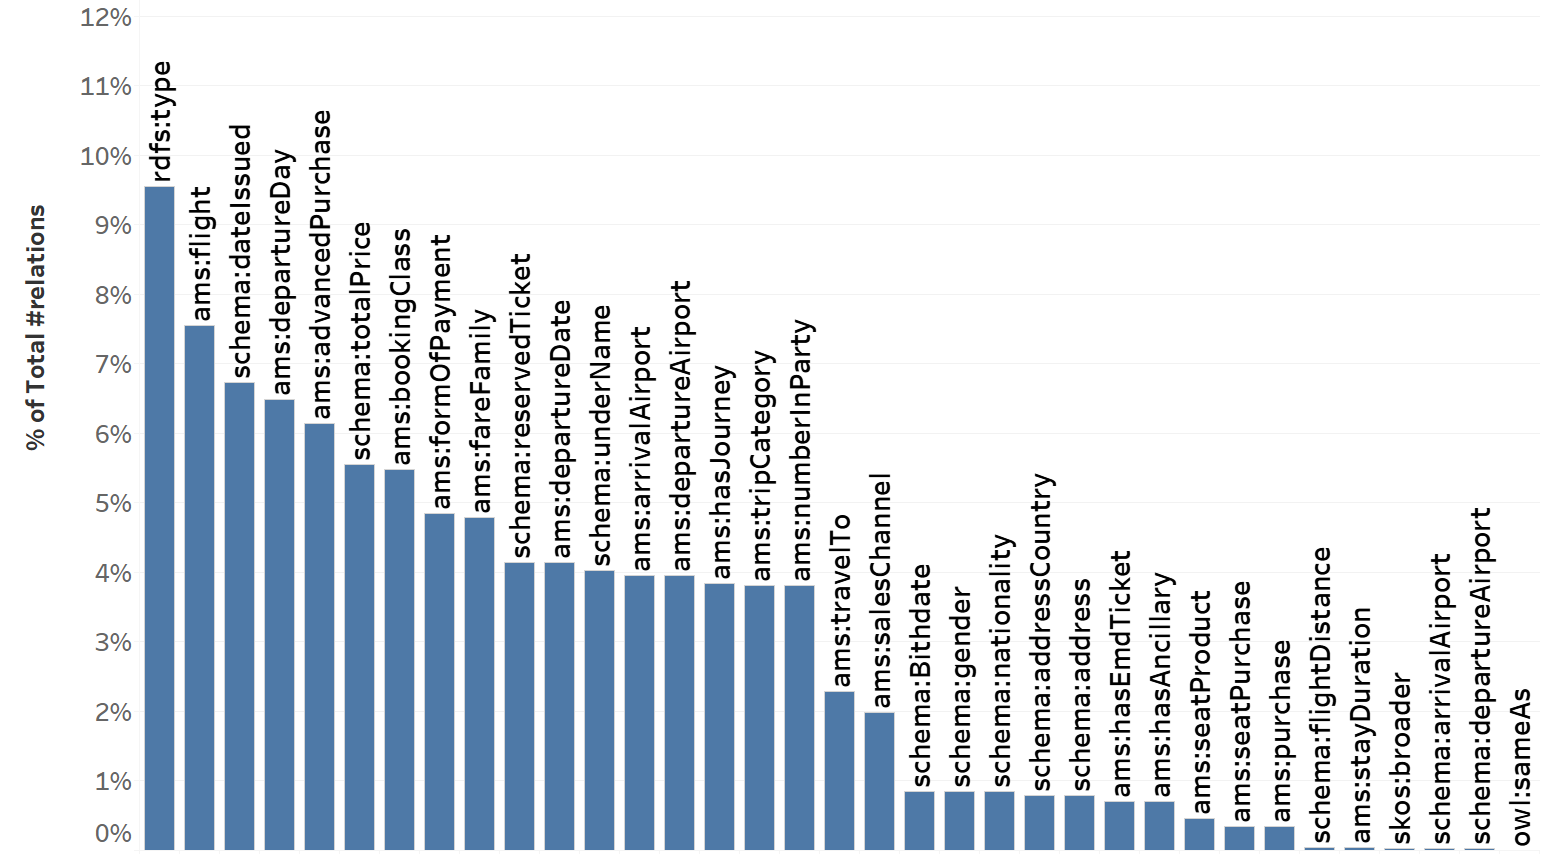
\includegraphics[width=1.05\linewidth]{figs/Properties_Distribution.png}
  \caption{Distribution of \#relations of properties in the Airline Travel KG. All prefixes can be found in the ontology definition.}
  \label{fig:properties}
\end{figure}

We present in Table \ref{tab:subgraphs} some statistics about the Airline Travel KG. 
\begin{table}[htbp]
  \centering
  \caption{Statistics of subgraphs}
  \label{tab:subgraphs}
  \footnotesize
  \begin{tabular}{|c|c|c|c|c|}
    \hline
    Subgraph & \#Edges & \#Nodes & \#travelers & \#PNRs\\
    \hline
    Extra leg room seat & 7M & 800K & 67K & 205K \\
    \hline
    Prepaid baggage & 64M & 7.6M & 572K & 2.2M \\
    \hline
    Lounge & 6.7M & 789K & 42K & 203K \\
  \hline
\end{tabular}
\end{table}
In Figure~\ref{fig:kg}, an excerpt of the KG is depicted, where a Malaysian traveler identified by T21354, born on "1988-05-05" has booked a one way flight for two people from Kuala lumpur to Melbourne. The EMD ticket identified by 23143 and linked to the air ticket 21563 represents the purchase of an ancillary (a seat).
\begin{figure*}[hbt!]
  \centering
  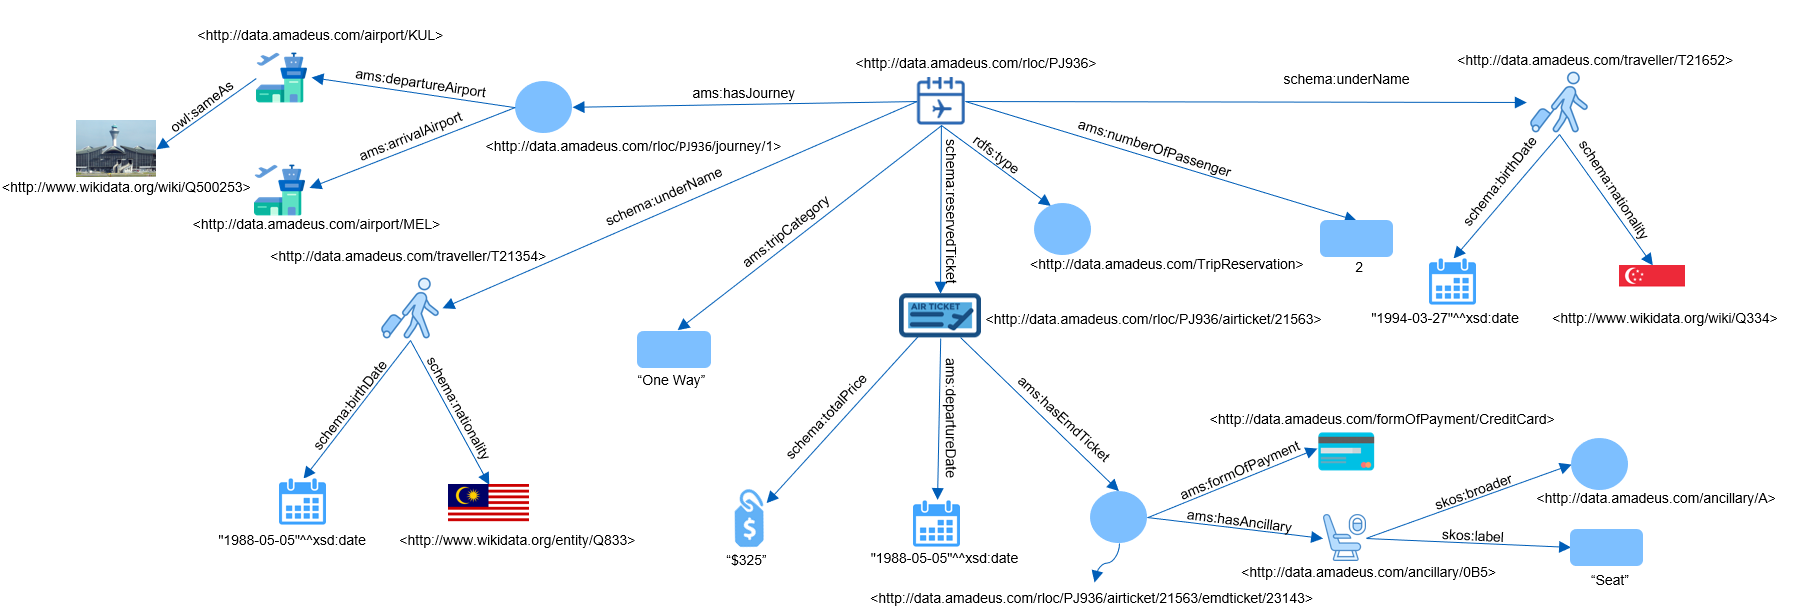
\includegraphics[width=\linewidth, height=6.5 cm]{figs/Airline_Travel_KG.png}
  \caption{Excerpt of the knowledge graph representing the travelers included in a Trip reservation through the property \texttt{schema:underName}, as well as other properties and relations to other entities. Literals are represented in blue rectangle, whereas other entities are represented in blue circle. In this depiction, some properties that links travelers, trip reservations, air tickets and emd tickets are represented as an example, but more properties are included in the graph.}
  \label{fig:kg}
\end{figure*}

\section{Approach}
\label{sec:approach}
Our proposed framework TKE can be seen as a two-stage approach as presented in Figure~\ref{fig:TKE-approach}. In the first stage, we extract contextual features from the ATN dataset and compute KG embeddings of travelers and trip reservations from the Airline Travel KG. In the second stage, contextual features and KG embeddings are used as input of an XGBoost classifier in order to predict, for a given user, whether the notification should be sent or not.

We also propose a supervised machine learning model that includes as input contextual features and additional handcrafted travelers' features that capture travelers' preferences which we think could be particularly significant for model accuracy (hypothesis proven in the ablation study) as another baseline to compare with. We describe below the handcrafted travelers' features as well as the KG embeddings used in TKE:
\begin{itemize}
    \item \textbf{Handcrafted travelers' features}: Features designed to capture travelers' preferences for ancillaries, destinations, points of sale, etc. and also customer lifetime value (Section~\ref{subsec:handcrafted}). 
    \item \textbf{Knowledge graph embeddings}: Latent features representation of travelers and trip reservations computed based on KG embedding algorithms such as TransE~\cite{bordes13} (Section~\ref{subsec:embeddings}). 
\end{itemize}

\subsection{Handcrafted Travelers Features}
\label{subsec:handcrafted}
In this section, we present the handcrafted travelers features designed to compare their use with that of KG embeddings. We compute several features based on travelers purchase history, such as preferred ancillary, preferred destination, etc. We list below the features computed that leverage travelers' history:
\begin{itemize}
    \item \textit{Bookings count}: Number of bookings already purchased by the traveler with the airline.
    \item \textit{Average flight revenue}: The average booking price tickets for all historical bookings of the traveler.
    \item \textit{Preferred ancillary}: This feature corresponds to the most sold ancillary to the traveler.
    \item \textit{Preferred destination}: This feature corresponds to the most visited destination (airport) by the traveler.
    \item \textit{Preferred seat characteristic}: This feature represents the seat characteristic that is the most purchased by the traveler. There are three types of seat characteristic namely Upper deck, Exit Row, Leg Space. 
    \item \textit{Extra leg room seat already purchase}: For each seat characteristic, we create a binary feature that represents if a traveler has already purchased an Extra leg room seat or not.
    \item \textit{Seat sales count}: This feature represents the number of times a seat has been purchased by the traveler.
    \item \textit{Prepaid baggage sales count}: This feature represents the number of times a prepaid baggage has been purchased by the traveler.
    \item \textit{Lounge sales count}: This feature represents the number of times a lounge access has been purchased by the traveler.
    \item \textit{Notification response rate}: This feature is equal to the number of sales divided by the number of notifications sent to the traveler (regardless of the recommended service).
\end{itemize}

The handcrafted features and the features available in the ATN dataset are used as input of a gradient boosting decision tree classifier. We use the official implementation\footnote{\url{XGBoost: https://XGBoost.readthedocs.io/}} of XGBoost~\cite{Chen16} to train a binary classifier to predict if the notified travelers will convert or not. In Section \ref{sec:experiments}, we give more details about the hyper-parameters used in XGBoost.

\subsection{TKE Features}
\label{subsec:embeddings}
In this section, we explain how the KG embeddings used in TKE are computed. We use translational distance models to compute travelers and trip reservations embeddings as shown in Figure~\ref{fig:TKE-approach}. More formally, we learn the KG embeddings based on a link prediction task, where some links of ancillary purchases and seat products are hidden in the training set, and put in the test set. Translational distance models are trained under the closed world assumption~\cite{Wang18} using a pairwise loss that penalizes negative instances. More concretely, ancillaries that were not purchased by a traveler are considered as negative instances under the closed world assumption. Translational distance models are evaluated using ranking metrics such as hit rate or mean reciprocal rank. Hence, these models will return a high similarity score (low euclidean distance) for the ancillaries that are close in the graph embedding space to the embeddings of the ancillaries historically purchased by the travelers. As an example, we obtain a hit rate of $\sim 0.42$ with the TransE algorithm on the Airline Travel KG. In addition to translational distance models, we implemented a single-hidden multi-layer perceptron (MLP) as proposed in~\cite{Xin14}, where each relation (as well as entity) is associated with a single vector. More specifically, given a fact (h, r, t), the vector embeddings of h, r, and t are concatenated in the input layer, and mapped to a non-linear hidden layer. The score is then generated by a linear output layer. The generated embeddings are used as input of XGBoost classifier in addition to the contextual features as shown in Figure~\ref{fig:TKE-approach}. We carry out a thorough empirical comparison of the aforementioned KG embedding algorithms and select the KG embeddings that allow the classifier to predict with the highest accuracy.

\section{Experiments}
\label{sec:experiments}
The objective of the experiments is to compare the use of handcrafted features (a) with the use of KG embeddings (b). (a) helps in interpreting the results and predictions obtained by the algorithm, while (b) lacks interpretation (latent features), but is easier to compute and maintain. We publish our code as open source in order to ease reproducibility\footnote{\url{https://gitlab.eurecom.fr/amadeus/tke4rec}}.

\begin{table*}[htbp]
  \centering
  \caption{Evaluation results of the different approaches. (a) represents the results of XGBoost for different inputs; (b) represents the results of the TKE approach for different KG embedding algorithms. The average standard deviation (by varying the seed when splitting the dataset) of each metric is as follows: $AUC-ROC: \pm 0.02$, $TPR : \pm 3\%$, $TNR : \pm 2\%$, $CR : \pm 0.1\%$}
  \label{tab:results}
  \begin{tabular}{|p{1.8 cm}|p{0.8 cm}p{0.8 cm}p{0.8 cm}p{0.8 cm}|p{0.8 cm}p{0.8 cm}p{0.8 cm}p{0.8 cm}|p{0.8 cm}p{0.8 cm}p{0.8 cm}p{0.8cm}|}
    \hline
    \multirow{2}{*}{Model} & \multicolumn{4}{c|}{Extra leg room seat} &  \multicolumn{4}{c|}{Prepaid baggage} & \multicolumn{4}{c|}{Lounge} \\
     & AUC-ROC & TPR & TNR & CR & AUC-ROC & TPR & TNR & CR & AUC-ROC & TPR & TNR & CR \\
    \hline
    Rule-based & - & - & - & 0.8\% & - & - & - & 0.15\% & - & - & - & 0.03\% \\
    \hline
    (a) ADS & 0.75 & 78\% & 58\% & 2.2\% & 0.83 & 80\% & 71\% & 0.38\% & 0.76 & 80\% & 62\% & 0.18\% \\
    (a) HDS & 0.79 & 81\% & 60\% & 2.37\% & 0.85 & 82\% & 74\% & 0.4\% & 0.84 & 86\% & 67\% & 0.22\% \\
    (a) AHDS & 0.83 & 85\% & 65\% & 2.8\% & 0.88 & 86\% & \textbf{74}\% & 0.56\% & 0.89 & 88\% & 65\% & 0.36\% \\
    \hline
    (b) TransE & 0.85 & 86\% & 69\% & 3.1\% & 0.91 & 92\% & 65\% & 0.6\% & 0.90 & 89\% & 78\% & 0.35\% \\
    (b) TransH & 0.84 & 85\% & 67\% & 3\% & 0.90 & 91\% & 65\% & 0.59\% & \textbf{0.95} & \textbf{96\%} & \textbf{85\%} & \textbf{0.59}\% \\
    (b) TransR & 0.84 & 85\% & 67\% & 2.9\% & 0.90 & 91\% & 65\% & 0.6\% & 0.92 & 92\% & 80\% & 0.52\% \\
    (b) MLP & \textbf{0.87} & \textbf{88\%} & \textbf{69\%} & \textbf{3.2\%} & \textbf{0.92} & \textbf{94\%} & 65\% & \textbf{0.62\%} & 0.91 & 90\% & 81\% & 0.56\% \\
    \hline
\end{tabular}
\end{table*}

\subsection{Experimental Setup}
\label{subsec:exp-setup}
In this section, we present the different settings and the evaluation protocol (evaluation metrics and split of the dataset) used to conduct the experiments.

\textbf{Dataset:} We experiment both approaches (a) and (b) with the three datasets presented in Table~\ref{tab:Notif_Conversion}. We use the Airline Travel KG presented in Section~\ref{subsec:kg} to generate the KG embeddings useful for our main approach TKE.

\textbf{Training \& Test Sets:} The three datasets corresponding to the three notification campaigns are split using the same strategy. Each dataset is sorted temporally, and 80\% of the first rows of each dataset are used as training/validation sets. We use a cross-fold validation to train and validate all models (k=5, a split of 80\% for training and 20\% for validation). The remaining 20\% are used as test set to evaluate the model. The split between training and validation set is performed randomly in order to avoid a seasonality effect that is usually occurring in the travel industry. KG embedding algorithms are often designed to solve a link prediction task. We consider it is appropriate to split the KG by removing some edges that are included in the set of properties that link travelers with ancillaries and consider them as test sets, in order to evaluate the quality of the computed embeddings.

\textbf{Evaluation metrics:} The output of our approach is the probability of purchasing the recommended ancillary $a$ included in the notification $N$:
\begin{equation}
    P(purchase = a|N) = P(purchase|Context, TE, RE)
\end{equation}
where, $TE$ and $RE$ are the Traveler and Trip reservation embeddings.

To evaluate and compare, the different approaches implemented, we used the conversion rate defined at definition~\ref{def:CR} and the three metrics defined as follows: 
\begin{itemize}
 \item \textbf{TPR}: The true positive rate is the percentage of correct positive predictions. It represents the ratio of travelers that the algorithm suggests to send the notification and effectively purchase the ancillary. TPR is defined as follows:
    \begin{equation}
        TPR = \frac{TP}{(TP+FN)}
    \end{equation}
 \item \textbf{TNR}: The true negative rate is the percentage of correct negative predictions. It represents the ratio of travelers that the algorithm suggest to not send the notification and effectively do not purchase the ancillary. TNR is defined as follows:
    \begin{equation}
        TNR = \frac{TN}{(TN+FP)}
    \end{equation}
 \item \textbf{ROC-AUC}: The area under ROC curve (FPR, TPR) helps to choose what is the optimal probability threshold that maximizes the CR and TPR and is defined as follows:
    \begin{equation}
        ROC\textrm{-}AUC = \int_{0}^{1} TPR \; d(FPR)
    \end{equation}
 where, $FPR = 1-TPR$ is the false positive rate
\end{itemize}

It is noteworthy that the conversion rate was measured offline as well as all the metrics based on the test set. According to equation~\ref{eq:CR}, $N_{o}$ represents the number of predicted positives and each hit $hit_{i}$ corresponds to a true positive prediction.

\textbf{Implementation Framework \& Parameter Settings:} For KG embedding algorithms, we use the deep learning framework pytorch\footnote{\url{Pytorch: https://pytorch.org/}} to implement MLP~\cite{Xin14} and the library pykg2vec~\cite{Yu19} for all the other KG embedding algorithms. The hyper-parameters of all the models were tuned using a combination of random-search and grid-search algorithms. We apply grid-search algorithm on the implemented algorithms using the following values: the embedding size k $ \in \{32, 64, ,96, 128, 256\}$, the batch size $\in \{128, 256, 512, 1024\}$, the number of epochs $\in \{50, 100, 200\}$, the learning rate lr $\in \{0.001,\\ 0.003, 0.01, 0.03, 0.1, 0.3\}$ and negative samples Ns $\in [2, 10]$ for MLP algorithm. We also optimize the following hyper-parameters of XGBoost classifier: the max depth of a tree $\in [5, 50]$, the number of trees $\in [10, 100]$, the sub-sample of each tree $\in [0.65, 0.85]$ and the col-sample of each tree $\in [0.65, 0.85]$. In addition to these hyper-parameters, we compute a weighted score (ratio of number of negative class to the positive class) that we use in XGBoost to approach the problem as a cost-sensitive learning problem due to the high class imbalance between positive (purchase) and negative (no purchase) classes (Table~\ref{tab:Notif_Conversion}).

\subsection{Results and Discussion}
\label{subsec:res-discussion}
In this section, we discuss the results obtained from the experiments. Results of the experiments conducted are presented in table~\ref{tab:results}. TPR, TNR and ROC-AUC metrics are not provided for the rule-based approach implemented in AAM Notification System. The reason behind this is that the dataset used in the experiments is generated by the AAM notification system, which is different from the original dataset that contains all travelers used for the rule-based approach to identify the travelers matching the targeting criteria.

\textbf{Ablation Study:}
Table~\ref{tab:results} shows that using the features from the ATN dataset in addition to the travelers handcrafted features (AHDS: ATN + Handcrafted features) as input of XGBoost performs better than using only one of them (ADS: ATN features or HDS: Handcrafted features) as input for all notification campaigns. We also observe that using only travelers handcrafted features as input information of XGBoost gives better results than using the entire ATN dataset for all notification campaigns. We compute the most important features of the model (a) AHDS for each notification campaign and we report below the three most important ones with their respective information gain:

\begin{itemize}
    \item Extra Leg Room Seat: \{\textit{Preferred Seat Characteristic}: 0.31,  \textit{Preferred ancillary}: 0.12,  \textit{Ticket amount}: 0.08\}.
    \item Prepaid Baggage: \{\textit{Preferred destination}: 0.21,  \textit{Destination}: 0.12,  \textit{Prepaid Baggage sales Frequency}: 0.10\}.
    \item Lounge: \{\textit{Average Flight Revenue}: 0.22,  \textit{Destination}: 0.20,  \textit{Age}: 0.15\}.
\end{itemize}

\textbf{Knowledge graph embeddings:}
We observe in Table~\ref{tab:results} that using KG embeddings (concatenation of traveler and reservation KG embeddings) with contextual features as input of XGBoost performs better than using travelers handcrafted features regardless of the algorithm used to compute the embeddings or the notification campaign. Moreover, KG embeddings computed from \textbf{MLP} shows to perform better than KG embeddings computed from translational distance models except for the lounge notification campaign, where the use of KG embeddings computed from \textbf{TransH} model gives the best results. 

\section{Conclusions and Future Work}
\label{sec:conclusion}
In this work, we have presented a two stage approach to address the problem of audience targeting for email marketing campaigns: first, we compute KG embeddings of travelers and reservations; second, we use these embeddings in addition to contextual features as input of a XGBoost classifier to learn what is the relevant audience to target for a given notification campaign. We conducted several experiments to address our research questions:

\textbf{RQ 1}: The results of the experiments presented in Table~\ref{tab:results} show that extracting the relevant audience for a given notification campaign is not an easy task. Indeed, despite the fact that the conversion rate increases significantly with our approach, it remains relatively small. However, thanks to our approach, notification campaigns are better targeted and we manage to avoid recommending an unsuitable service to at least 65\% of passengers. 

\textbf{RQ 2}: Experiments have shown that the handcrafted features based supervised machine learning approach (a) gives better results than the rule-based one. Indeed, in Table~\ref{tab:results}, we can observe that the conversion rate is multiplied by more than 3 for Extra Leg Room Seat, almost 4 for Prepaid Baggage, and 12 for Lounge. Hence, we prove the benefit of using supervised machine learning over a simpler rule-based approach while it is the currently adopted mechanism used by airline marketers. It should be noted that the list of possible criteria available in AAM Notification System (Figure~\ref{fig:TKE-approach}) is the same as the list of features used in the supervised machine learning approach. 

\textbf{RQ 3}: Experiments show that regardless of the KG embedding algorithm tested, the KG embedding approach is better than the handcrafted features approach. This is very interesting from a scientific point of view, as it shows the added value of having a KG in the travel domain that could be used not only for ancillary recommendation task, but also other recommendation tasks (e.g. Trip recommendation) as the same KG embeddings could be used. It is worth noticing that when dealing with a cold-start problem (new user or item) for on-line usability, a rule-based approach is more appropriate.

Finally, as future work, we expect to tackle the task of personalized ancillary ranking in email marketing campaigns. More specifically, the goal of our future work will be to answer what is the most appropriate service to recommend in a notification campaign. In addition to addressing and optimizing what to recommend to a traveler, it would be interesting to optimize the time when to send the notification as it is an important decision making factor, especially in the airline travel industry~\cite{Dadoun21}.


%Bibliography.
% Generated by IEEEtran.bst, version: 1.14 (2015/08/26)
\begin{thebibliography}{10}
\providecommand{\url}[1]{#1}
\csname url@samestyle\endcsname
\providecommand{\newblock}{\relax}
\providecommand{\bibinfo}[2]{#2}
\providecommand{\BIBentrySTDinterwordspacing}{\spaceskip=0pt\relax}
\providecommand{\BIBentryALTinterwordstretchfactor}{4}
\providecommand{\BIBentryALTinterwordspacing}{\spaceskip=\fontdimen2\font plus
\BIBentryALTinterwordstretchfactor\fontdimen3\font minus
  \fontdimen4\font\relax}
\providecommand{\BIBforeignlanguage}[2]{{%
\expandafter\ifx\csname l@#1\endcsname\relax
\typeout{** WARNING: IEEEtran.bst: No hyphenation pattern has been}%
\typeout{** loaded for the language `#1'. Using the pattern for}%
\typeout{** the default language instead.}%
\else
\language=\csname l@#1\endcsname
\fi
#2}}
\providecommand{\BIBdecl}{\relax}
\BIBdecl

\bibitem{Dadoun21}
A.~Dadoun, T.~Fiig, M.~Defoin-Platel, C.~Landra, and R.~Troncy, ``How
  recommender systems can transform airline offer construction and retailing,''
  \emph{Journal of Revenue and Pricing Management, Special issue on AI}, 2021.

\bibitem{Palumbo18}
E.~Palumbo, G.~Rizzo, R.~Troncy, E.~Baralis, M.~Osella, and E.~Ferro,
  ``Translational models for item recommendation,'' in \emph{The Semantic Web:
  ESWC 2018 Satellite Events}, A.~Gangemi, A.~L. Gentile, A.~G. Nuzzolese,
  S.~Rudolph, M.~Maleshkova, H.~Paulheim, J.~Z. Pan, and M.~Alam, Eds.\hskip
  1em plus 0.5em minus 0.4em\relax Cham: Springer International Publishing,
  2018, pp. 478--490.

\bibitem{Sun18}
Z.~Sun, J.~Yang, J.~Zhang, A.~Bozzon, L.-K. Huang, and C.~Xu, ``{Recurrent
  Knowledge Graph Embedding for Effective Recommendation},'' in \emph{12th ACM
  Conference on Recommender Systems}.\hskip 1em plus 0.5em minus 0.4em\relax
  New York, NY, USA: ACM, 2018, pp. 297--305.

\bibitem{Palumbo20}
E.~Palumbo, D.~Monti, G.~Rizzo, R.~Troncy, and E.~Baralis, ``entity2rec:
  Property-specific knowledge graph embeddings for item recommendation,''
  \emph{Expert Syst. Appl.}, vol. 151, p. 113235, 2020.

\bibitem{Pawel19}
P.~Jankiewicz, L.~Kyrashchuk, P.~Sienkowski, and M.~W\'{o}jcik, ``Boosting
  algorithms for a session-based, context-aware recommender system in an online
  travel domain,'' in \emph{Proceedings of the Workshop on ACM Recommender
  Systems Challenge}, ser. RecSys Challenge '19.\hskip 1em plus 0.5em minus
  0.4em\relax New York, NY, USA: Association for Computing Machinery, 2019.

\bibitem{Schifferer20}
\BIBentryALTinterwordspacing
B.~Schifferer, G.~Titericz, C.~Deotte, C.~Henkel, K.~Onodera, J.~Liu,
  B.~Tunguz, E.~Oldridge, G.~De~Souza Pereira~Moreira, and A.~Erdem, ``Gpu
  accelerated feature engineering and training for recommender systems,'' in
  \emph{Proceedings of the Recommender Systems Challenge 2020}, ser.
  RecSysChallenge '20.\hskip 1em plus 0.5em minus 0.4em\relax New York, NY,
  USA: Association for Computing Machinery, 2020, pp. 16--23. [Online].
  Available: \url{https://doi.org/10.1145/3415959.3415996}
\BIBentrySTDinterwordspacing

\bibitem{Chittenden2003}
L.~Chittenden and R.~Rettie, ``An evaluation of e-mail marketing and factors
  affecting response,'' \emph{Journal of Targeting, Measurement and Analysis
  for Marketing}, vol.~11, pp. 203--217, 2003.

\bibitem{Sahni17}
\BIBentryALTinterwordspacing
N.~S. Sahni, D.~Zou, and P.~K. Chintagunta, ``Do targeted discount offers serve
  as advertising? evidence from 70 field experiments,'' \emph{Manage. Sci.},
  vol.~63, no.~8, pp. 2688--2705, Aug. 2017. [Online]. Available:
  \url{https://doi.org/10.1287/mnsc.2016.2450}
\BIBentrySTDinterwordspacing

\bibitem{Abakouy17}
\BIBentryALTinterwordspacing
R.~Abakouy, E.~M. En-Naimi, and A.~El~Haddadi, ``Classification and prediction
  based data mining algorithms to predict email marketing campaigns,'' in
  \emph{Proceedings of the 2nd International Conference on Computing and
  Wireless Communication Systems}, ser. ICCWCS'17.\hskip 1em plus 0.5em minus
  0.4em\relax New York, NY, USA: Association for Computing Machinery, 2017.
  [Online]. Available: \url{https://doi.org/10.1145/3167486.3167520}
\BIBentrySTDinterwordspacing

\bibitem{Deligiannis2020}
\BIBentryALTinterwordspacing
A.~Deligiannis, C.~Argyriou, and D.~Kourtesis, ``Predicting the optimal date
  and time to send personalized marketing messages to repeat buyers,''
  \emph{International Journal of Advanced Computer Science and Applications},
  vol.~11, no.~4, 2020. [Online]. Available:
  \url{http://dx.doi.org/10.14569/IJACSA.2020.0110413}
\BIBentrySTDinterwordspacing

\bibitem{Tamho05}
\BIBentryALTinterwordspacing
K.~Y. Tam and S.~Y. Ho, ``Web personalization as a persuasion strategy: An
  elaboration likelihood model perspective,'' \emph{Info. Sys. Research},
  vol.~16, no.~3, pp. 271--291, Sep. 2005. [Online]. Available:
  \url{https://doi.org/10.1287/isre.1050.0058}
\BIBentrySTDinterwordspacing

\bibitem{Yang19}
K.~Yang, J.~H. Min, and K.~Garza-Baker, ``Post-stay email marketing
  implications for the hotel industry: Role of email features, attitude,
  revisit intention and leisure involvement level,'' \emph{Journal of Vacation
  Marketing}, vol.~25, no.~4, pp. 405--417, 2019.

\bibitem{Wang18}
Q.~Wang, Z.~Mao, B.~Wang, and L.~Guo, ``Knowledge graph embedding: A survey of
  approaches and applications,'' \emph{IEEE Transactions on Knowledge and Data
  Engineering}, vol.~29, no.~12, pp. 2724--2743, Dec 2017.

\bibitem{bordes13}
\BIBentryALTinterwordspacing
A.~Bordes, N.~Usunier, A.~Garcia-Duran, J.~Weston, and O.~Yakhnenko,
  ``Translating embeddings for modeling multi-relational data,'' in
  \emph{Advances in Neural Information Processing Systems 26}, C.~J.~C. Burges,
  L.~Bottou, M.~Welling, Z.~Ghahramani, and K.~Q. Weinberger, Eds.\hskip 1em
  plus 0.5em minus 0.4em\relax Red Hook, NY, USA: Curran Associates, Inc.,
  2013, pp. 2787--2795. [Online]. Available:
  \url{http://papers.nips.cc/paper/5071-translating-embeddings-for-modeling-multi-relational-data.pdf}
\BIBentrySTDinterwordspacing

\bibitem{Wang14}
Z.~Wang, J.~Zhang, J.~Feng, and Z.~Chen, ``Knowledge graph embedding by
  translating on hyperplanes,'' in \emph{Proceedings of the Twenty-Eighth AAAI
  Conference on Artificial Intelligence}, ser. AAAI'14.\hskip 1em plus 0.5em
  minus 0.4em\relax Qu\'{e}bec City, Qu\'{e}bec, Canada: AAAI Press, 2014, pp.
  1112--1119.

\bibitem{Yankai15}
Y.~Lin, Z.~Liu, M.~Sun, Y.~Liu, and X.~Zhu, ``Learning entity and relation
  embeddings for knowledge graph completion,'' in \emph{Proceedings of the
  Twenty-Ninth AAAI Conference on Artificial Intelligence}, ser. AAAI'15.\hskip
  1em plus 0.5em minus 0.4em\relax Austin, Texas: AAAI Press, 2015, pp.
  2181--2187.

\bibitem{Maximilian11}
M.~Nickel, V.~Tresp, and H.-P. Kriegel, ``A three-way model for collective
  learning on multi-relational data,'' in \emph{Proceedings of the 28th
  International Conference on International Conference on Machine Learning},
  ser. ICML'11.\hskip 1em plus 0.5em minus 0.4em\relax Madison, WI, USA:
  Omnipress, 2011, pp. 809--816.

\bibitem{Palumbo17}
E.~Palumbo, G.~Rizzo, and R.~Troncy, ``Entity2rec: Learning user-item
  relatedness from knowledge graphs for top-n item recommendation,'' in
  \emph{Eleventh ACM Conference on Recommender Systems}.\hskip 1em plus 0.5em
  minus 0.4em\relax New York, NY, USA: ACM, 2017, pp. 32--36.

\bibitem{Aditya16}
A.~Grover and J.~Leskovec, ``Node2vec: Scalable feature learning for
  networks,'' in \emph{22Nd ACM SIGKDD International Conference on Knowledge
  Discovery and Data Mining}.\hskip 1em plus 0.5em minus 0.4em\relax New York,
  NY, USA: ACM, 2016, pp. 855--864.

\bibitem{Chen16}
T.~Chen and C.~Guestrin, ``Xgboost: A scalable tree boosting system,'' in
  \emph{22$^{nd}$ ACM SIGKDD International Conference on Knowledge Discovery
  and Data Mining (KDD)}.\hskip 1em plus 0.5em minus 0.4em\relax San Francisco,
  California, USA: Association for Computing Machinery, 2016, pp. 785--794.

\bibitem{Dadoun19}
A.~Dadoun, R.~Troncy, O.~Ratier, and R.~Petitti, ``{Location Embeddings for
  Next Trip Recommendation},'' in \emph{9$^{th}$ International Workshop on
  Location on the Web (LocWeb)}.\hskip 1em plus 0.5em minus 0.4em\relax San
  Francisco, USA: Association for Computing Machinery, 2019, pp. 896--903.

\bibitem{Xin14}
\BIBentryALTinterwordspacing
X.~Dong, E.~Gabrilovich, G.~Heitz, W.~Horn, N.~Lao, K.~Murphy, T.~Strohmann,
  S.~Sun, and W.~Zhang, ``Knowledge vault: A web-scale approach to
  probabilistic knowledge fusion,'' in \emph{Proceedings of the 20th ACM SIGKDD
  International Conference on Knowledge Discovery and Data Mining}, ser. KDD
  '14.\hskip 1em plus 0.5em minus 0.4em\relax New York, NY, USA: Association
  for Computing Machinery, 2014, pp. 601--610. [Online]. Available:
  \url{https://doi.org/10.1145/2623330.2623623}
\BIBentrySTDinterwordspacing

\bibitem{Yu19}
\BIBentryALTinterwordspacing
S.-Y. Yu, S.~R. Chhetri, A.~Canedo, P.~Goyal, and M.~A.~A. Faruque, ``Pykg2vec:
  A python library for knowledge graph embedding,'' \emph{Journal of Machine
  Learning Research}, vol.~22, no.~16, pp. 1--6, 2021. [Online]. Available:
  \url{http://jmlr.org/papers/v22/19-433.html}
\BIBentrySTDinterwordspacing

\end{thebibliography}



\end{document}